% This template has been tested with LLNCS DOCUMENT CLASS -- version 2.20 (24-JUN-2015)

%"runningheads" enables:
%  - page number on page 2 onwards
%  - title/authors on even/odd pages
%This is good for other readers to enable proper archiving among other papers and pointing to content.
%Even if the title page states the title, when printed and stored in a folder, when blindly opening the folder, one could hit not the title page, but an arbitrary page. Therefore, it is good to have title printed on the pages, too.
\documentclass[runningheads,a4paper]{llncs}[2015/06/24]

%Even though `american`, `english` and `USenglish` are synonyms for babel package (according to https://tex.stackexchange.com/questions/12775/babel-english-american-usenglish), the llncs document class is prepared to avoid the overriding of certain names (such as "Abstract." -> "Abstract" or "Fig." -> "Figure") when using `english`, but not when using the other 2.
\usepackage[english]{babel}

%better font, similar to the default springer font
%cfr-lm is preferred over lmodern. Reasoning at http://tex.stackexchange.com/a/247543/9075
\usepackage[%
rm={oldstyle=false,proportional=true},%
sf={oldstyle=false,proportional=true},%
tt={oldstyle=false,proportional=true,variable=true},%
qt=false%
]{cfr-lm}
%
%if more space is needed, exchange cfr-lm by mathptmx
%\usepackage{mathptmx}

\usepackage{graphicx}


%% If you need packages for other papers,
%% START COPYING HERE

%extended enumerate, such as \begin{compactenum}
\usepackage{paralist}

\usepackage{amsmath}
%put figures inside a text
%\usepackage{picins}
%use
%\piccaptioninside
%\piccaption{...}
%\parpic[r]{\includegraphics ...}
%Text...

%Sorts the citations in the brackets
%It also allows \cite{refa, refb}. Otherwise, the document does not compile.
%  Error message: "White space in argument"
\usepackage{cite}

\usepackage[T1]{fontenc}
\usepackage{cmap}

%for demonstration purposes only
\usepackage[math]{blindtext}

%for easy quotations: \enquote{text}
\usepackage{csquotes}

%enable margin kerning
\usepackage{microtype}

%tweak \url{...}
\usepackage{url}
\urlstyle{same}
%improve wrapping of URLs - hint by http://tex.stackexchange.com/a/10419/9075
\makeatletter
\g@addto@macro{\UrlBreaks}{\UrlOrds}
\makeatother
%nicer // - solution by http://tex.stackexchange.com/a/98470/9075
%DO NOT ACTIVATE -> prevents line breaks
%\makeatletter
%\def\Url@twoslashes{\mathchar`\/\@ifnextchar/{\kern-.2em}{}}
%\g@addto@macro\UrlSpecials{\do\/{\Url@twoslashes}}
%\makeatother

%diagonal lines in a table - http://tex.stackexchange.com/questions/17745/diagonal-lines-in-table-cell
%slashbox is not available in texlive (due to licensing) and also gives bad results. This, we use diagbox
%\usepackage{diagbox}

%required for pdfcomment later
\usepackage{xcolor}

% new packages BEFORE hyperref
% See also http://tex.stackexchange.com/questions/1863/which-packages-should-be-loaded-after-hyperref-instead-of-before

%enable hyperref without colors and without bookmarks
\usepackage[
%   pdfauthor={},
%   pdfsubject={},
%   pdftitle={},
%   pdfkeywords={},
   bookmarks=false,
   colorlinks=true,
   allcolors=black,
   pdfstartview=Fit,
   breaklinks=true,
]{hyperref}
%enables correct jumping to figures when referencing
\usepackage[all]{hypcap}

%enable nice comments
\usepackage{pdfcomment}
\newcommand{\commentontext}[2]{\colorbox{yellow!60}{#1}\pdfcomment[color={0.234 0.867 0.211},hoffset=-6pt,voffset=10pt,opacity=0.5]{#2}}
\newcommand{\commentatside}[1]{\pdfcomment[color={0.045 0.278 0.643},icon=Note]{#1}}

%compatibality with packages todo, easy-todo, todonotes
\newcommand{\todo}[1]{\commentatside{#1}}
%compatiblity with package fixmetodonotes
\newcommand{\TODO}[1]{\commentatside{#1}}

%enable \cref{...} and \Cref{...} instead of \ref: Type of reference included in the link
\usepackage[capitalise,nameinlink]{cleveref}
%Nice formats for \cref
\crefname{section}{Sect.}{Sect.}
\Crefname{section}{Section}{Sections}

\usepackage{xspace}
%\newcommand{\eg}{e.\,g.\xspace}
%\newcommand{\ie}{i.\,e.\xspace}
\newcommand{\eg}{e.\,g.,\ }
\newcommand{\ie}{i.\,e.,\ }

%introduce \powerset - hint by http://matheplanet.com/matheplanet/nuke/html/viewtopic.php?topic=136492&post_id=997377
\DeclareFontFamily{U}{MnSymbolC}{}
\DeclareSymbolFont{MnSyC}{U}{MnSymbolC}{m}{n}
\DeclareFontShape{U}{MnSymbolC}{m}{n}{
    <-6>  MnSymbolC5
   <6-7>  MnSymbolC6
   <7-8>  MnSymbolC7
   <8-9>  MnSymbolC8
   <9-10> MnSymbolC9
  <10-12> MnSymbolC10
  <12->   MnSymbolC12%
}{}
\DeclareMathSymbol{\powerset}{\mathord}{MnSyC}{180}

% correct bad hyphenation here
\hyphenation{op-tical net-works semi-conduc-tor}


%% END COPYING HERE


\begin{document}

\title{Implementation of a Brute Force Attack on A5/1 Cryptographical
Algorithm in a GPU-based Volunteering Computing Project}
%If Title is too long, use \titlerunning
\titlerunning{A5/1 Brute Force on GPU}

%Single insitute
\author{Bulavintsev V. \and Semenov A. \and Zaikin O.}
%If there are too many authors, use \authorrunning
%\authorrunning{First Author et al.}
\institute{Matrosov Institute for System Dynamics and Control Theory of
Siberian Branch of Russian Academy of Sciences
(ISDCT SB RAS)}

%Multiple insitutes
%Currently disabled
%
\iffalse
%Multiple institutes are typeset as follows:
\author{Firstname Lastname\inst{1} \and Firstname Lastname\inst{2} }
%If there are too many authors, use \authorrunning
%\authorrunning{First Author et al.}

\institute{
Insitute 1\\
\email{...}\and
Insitute 2\\
\email{...}
}
\fi
			
\maketitle

\begin{abstract}
We present an advanced brute force attack on the A5/1 cryptoalgorithm,
	that is still broadly used in modern GSM networks. We use a
	well-known idea introduced by R.Anderson more than 20 years ago
	to greatly reduce the search space. The primary contribution of
	this article is the implementation of the Anderson's attack on a GPU platform
	with the bitslice technique. The preliminary estimates of the
	attack's speed showed that, with the use of a GPUs processing power, 
	the attack could be conducted in the real
	time on a modern computer cluster or in a volunteer computing
	project. To verify our estimates with the use of BOINC technology 
	we concieved the specialized volunteering computing project 
	and executed our variant of Anderson's attack within it. In the
	7 days the project lasted, 10 A5/1 cryptanalysis problems were
	solved. The results presented in this work provide yet another
	proof of A5/1's cryptographical weakness that make it totally
	unsuitable for transmission of any kind of sensitive data
	through modern GSM networks.

\end{abstract}

\begin{keywords}
A5/1 algorithm, brute-force cryptanalysis, GPU, volunteering computing
\end{keywords}

%%%%%%%%%%%%%%%%%%%%%%%%%%%%%%%%%%%%%%%%%%%%%%%%%%%%%%%%%%%%%%%%%%%%%%%%%%%%%%%
\section{Introduction}\label{sec:intro}
%%%%%%%%%%%%%%%%%%%%%%%%%%%%%%%%%%%%%%%%%%%%%%%%%%%%%%%%%%%%%%%%%%%%%%%%%%%%%%%
%\blindtext\todo{Refine me}

A5/1 algorithm is a keystream generator with key length of 64 bits. It is used
to encrypt voice and SMS traffic in 2nd generation ("2G") GSM networks. 3rd
generation GSM networks accept 2G communication protocol for backward
compatibility. A practice of sending voice traffic through 2G protocols in 3G
networks to conserve bandwith and increase service availability is widely
adopted among mobile phone operators. \todo{Can't find source} A widely adopted
practice among mobile operators is to still use 2G protocols to route voice
traffic even in 3rd generation GSM networks.

One can name A5/1 as one of the most publicly recognized cryptographical
algorithms, along with RSA and DES, it's discussion reaching far beyond the
borders of professional cryptographers community. For example, article
\cite{WASHPOST} publicly examines NSA's ability to efficiently decrypt A5/1.
So, in this article we won't touch on the details of A5/1's creation history
and the reasons of it's rise as the world's 'de facto' mobile communication
standard. Milestones in cryptanalysis of A5/1 would be briefly outlined in
Related Works section.

Among all the differrent methods of A5/1 cryptanalysis we distinguish those
which were realized in practice and allowed to reliably conduct the
cryptanalysis procedure on an non-weakened variant of algorithm. Apparently,
the first such attack was performed in 2008 with the help of the special
FPGA-based computational platform COPACOBANA\cite{COPAC_1}. In 2009 distributed
algorithms for boolean satisfiability (SAT) were used to solve several
cryptanalysis instances of stock A5/1 in a specialized grid system 'BNB-Grid'
\cite{TRUDY_ISA}. These results were further improved in 2011 \cite{SZBP}. By
the end of 2009 the 'A5/1 Cracking Project' had published rainbow tables
\cite{RAINBOW} for A5/1. Provided with 8 bursts (912 bits) of keystream these
tables allowed to find the secret key in less than a minute with more than 85\%
probabilty. Despite the huge (over 2 Tb) size, to this day these rainbow tables
provide the most practical method of A5/1 cryptanalysis.  It's main shortcoming
is that the probability of success is significantly less than 100\%. Meanwhile,
the growth of computational power of GPUs and FPGAs made practical the attack
based on reduction of search space from $2^64$ to $2^53$, which was described
by R.  Anderson in 1994. As was mentioned earlier, FPGA-based variant of the
Anderson's attack was already performed in 2008 by COPACOBANA creators. So, the
primary goal of our work is to demonstrate the viability of GPU-based variant
of the attack. Let us note that GPUs are much easier to operate than FPGAs, and
the former belong to the class of consumer-grade devices and could be found in
any modern PC, while the latter belong to the class of specialized equipment.
With the usage of the BOINC software platform \cite{BOINC_C}, this qualities of
GPUs allowed us to implement the attack in the form of a volunteering computing
project using idle computational capabilites of the project members home PCs.
Our estimates of attack's speed were based on our previous
work\cite{BUL_SEM_2016}.

Let's make a brief outline of the article's contents. In \Cref{sec:alg} we
describe the A5/1 algorithm along with some advanced brute-force attacks on it.
\Cref{sec:bitslc} introduces bit-slicing technique and goes through important
details of implementing the Anderson's attack with it. \Cref{sec:boinc}
provides a look into the internal organization of the volunteering project we
created for conducting the attack with GPUs. \Cref{sec:history} contains the
retrospective of A5/1 cryptanalysis works related to our study.


%%%%%%%%%%%%%%%%%%%%%%%%%%%%%%%%%%%%%%%%%%%%%%%%%%%%%%%%%%%%%%%%%%%%%%%%%%%%%%%
\section{A5/1 algorithm and some attack on it}\label{sec:alg}
%%%%%%%%%%%%%%%%%%%%%%%%%%%%%%%%%%%%%%%%%%%%%%%%%%%%%%%%%%%%%%%%%%%%%%%%%%%%%%%

A5/1 keystream generator consists of 3 linear feedback shift registers (LFSRs)
\cite{MENEZES}, defined by the following primitive polynomials:

\begin{gather*} X^{19}+X^{18}+X^{17}+X^{14}+1, LFSR1;\\X^{22}+X^{28}+1,
	LFSR2;\\ X^{23}+X^{22}+X^{21}+X^{8}+1, LFSR3.\end{gather*}

The illustration of A5/1 generator's work scheme can be seen at
\cref{fig:a5gen}.

\begin{figure}
	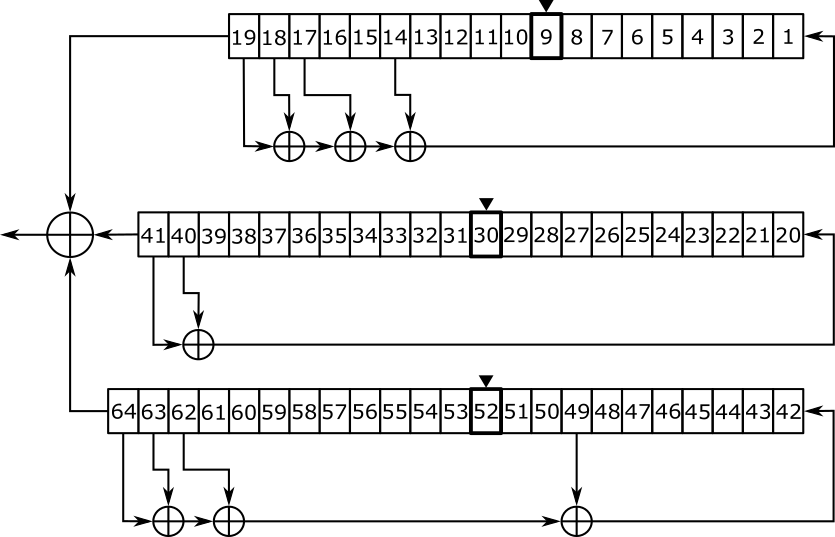
\includegraphics[width=\linewidth]{./a51.png} \caption{A5/1 generator work
scheme} \label{fig:a51gen} \end{figure}

The outputs of LFSRs are mixed with linear function, which provides the perfect
corellation immunity. Non-linearity of the equations is achieved by clocking
the registers asynchronously - for each clocking of the whole generator any of
the 3 registers could be clocked or it could retain it's current state.
Register with index $j \in \{1,2,3\}$ will be clocked if the following boolean
function $\chi_j$ becomes 1:

\begin {gather*} \chi_j = (b_j \equiv majority(b_1,b_2,b_3));
\\majority(A,B,C)=(A \wedge B) \vee (A \wedge C) \vee (B \vee C).
\end{gather*}

Here $b_1,b_2,b_3$ denote clocking bits marked at \cref{fig:a5gen} by black
wedges. Conversely, if at some moment $\chi_j=0$, LFSR $j$ won't clock (it will
remain in it's last state).

Generator A5/1 is used in the GSM protocol for high-speed encryption of large
volumes of information with the short secret key. The whole process is split
into 'sessions' about 3,5 hours long. Each session uses it's own 'session key'.
We won't touch on the topic of specialized protocols used in GSM networks to
build and transfer the session key.

Along the message data, GSM protocol sends error correction data for the
message. The message complete with error correction data constitutes a 456 bits
long 'frame', which is further broken down into 4 'bursts' of 114 bits. The
bursts are than encrypted and send over the air. To encrypt a burst the A5/1
generator is initialized with the 64-bit 'local key', that is built using
session key and a natural number called 'the frame number' (FN). After the
encryption of one burst is complete, the frame number is increased by 1. When
FN overflows, the session ends and a new session is initialized (hence the 3,5
session length). FN is always known from the open data transmitted over the
network. 

If the message length is less than 23 bytes, the message would be filled with
fixed pattern padding to 23 bytes. Some GSM technical messages used during the
voice call are fixed length and always padded. As padding is always the same,
and it is encrypted by some local key, we got a typical plain text attack
scenario at hand \cite{MENEZES}. Indeed, the padding plays the role of the
known plaintext, allowing the attacker to get the corresponding keystream
fragment. This vulnerability allows the attacker to get no less than two frames
(912 bits) of the keystream. It was demonstrated in \cite{UNKN1} that the
knowledge of even one local key and FN is enough to efficiently restore the
session key, which makes the decryption of the whole session possible.


The described vulnerability of GSM protocol allows to build some successful
attacks on it, based on the idea of 'advanced brute force'. In particular, the
large-scale preprocessing made possible the creation of the rainbow tables,
which, provided 8 bursts of keystream, allows to determine the session key with
probability in less than a minute with $>85\%$ probability. The tables take
about 2Tb of disk space. This attack is presented in detail in \cite{RAINBOW},
and still stands among the most practical ones. Instead, we will focus on the
idea of an attack that was suggested by Ross Anderson in 1994 in a small essay
on the A5/1 cryptographic strength \cite{COPAC}. Next we describe the essence
of the Anderson's attack.


\begin{figure} 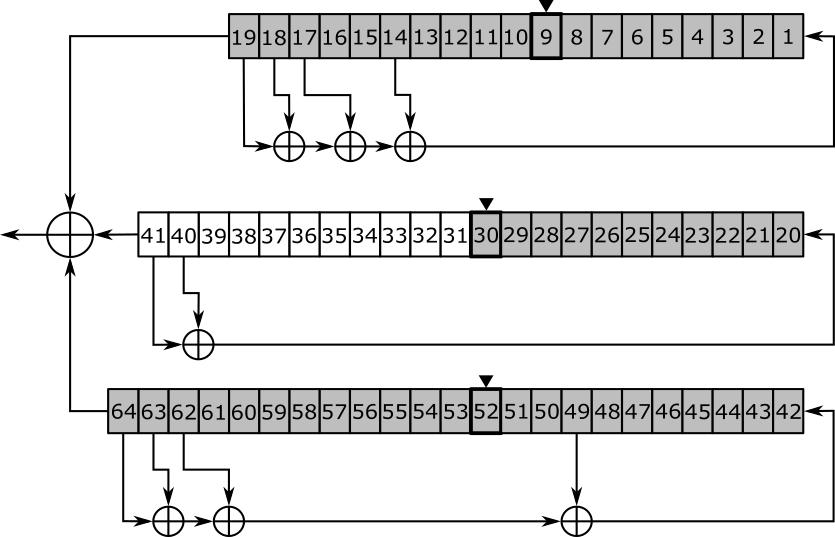
\includegraphics[width=\linewidth]{./a51and.png} \caption{The
	set of guessing bits used in Anderson's attack (greyed out).}
\label{fig:a51and} \end{figure}


Anderson's attack is a typical example of a 'guess and determine attack' (see
\cite{BARD}). Suppose we know the bits filling the 1st and the 3rd LFSR, and
bits of the 2nd LFSR from the beginning of the register to the clocking bit
(bits 31 to 41, see \cref{fig:a51and}). Next suppose we know 64 bits of the
keystream. Now, as was shown by R. Anderson, 11 unknown bits of the 2nd LFSR
could be figured out without any additional guesses. This happens because the
clocking bits are known (and so is the clocking schedule for the next 11
clockings of the 2nd LFSR), and known are 2 out of 3 XOR-ed LFSR output bits
and the result of the XOR operation (from the keystream). Therefore, one can
efficiently work out the unknown bits of the LFSR 2 one by one, by clocking the
generator and applying XOR operation to corresponding keystream bits and output
bits of LFSRs 1 and 3.

The description of the algorithm of determination of unknown 11 bits of LFSR 2
provided above makes obvious the possibility to mount a brute force attack on
the A5/1 generator over the search space of $2^{53}$. The simplicity of the
algorithm provides an opportunity to implement it on a specialized
computational architecture. One such implementation was built with FPGAs by
authors of \cite{COPAC_1}. In the following sections we describe our
implementation of this attack for modern GPUs.







Winery~\cite{Winery} is graphical \commentontext{modeling}{modeling with one \enquote{l}, because of AE} tool.

\begin{figure}
Simple Figure
\caption{Simple Figure}
\label{fig:simple}
\end{figure}

\begin{table}
\caption{Simple Table}

\label{tab:simple}
Simple Table
\end{table}

cref Demonstration: Cref at beginning of sentence, cref in all other cases.

\Cref{fig:simple} shows a simple fact, although \cref{fig:simple} could also show something else.

\Cref{tab:simple} shows a simple fact, although \cref{tab:simple} could also show something else.

\Cref{sec:intro} shows a simple fact, although \cref{sec:intro} could also show something else.

Brackets work as designed:
<test>

The symbol for powerset is now correct: $\powerset$ and not a Weierstrass p ($\wp$).

\begin{inparaenum}
\item All these items...
\item ...appear in one line
\item This is enabled by the paralist package.
\end{inparaenum}

``something in quotes'' using plain tex or use \enquote{the enquote command}.

\section{Conclusion and Outlook}

\subsubsection*{Acknowledgments}
...

In the bibliography, use \texttt{\textbackslash textsuperscript} for ``st'', ``nd'', ...:
E.g., \enquote{The 2\textsuperscript{nd} conference on examples}.
When you use \href{https://www.jabref.org}{JabRef}, you can use the clean up command to achieve that.

%%%%%%%%%%%%%%%%%%%%%%%%%%%%%%%%%%%%%%%%%%%%%%%%%%%%%%%%%%%%%%%%%%%%%%%%%%%%%%%
\bibliographystyle{splncs03}
\bibliography{paper}

All links were last followed on October 5, 2014.
%%%%%%%%%%%%%%%%%%%%%%%%%%%%%%%%%%%%%%%%%%%%%%%%%%%%%%%%%%%%%%%%%%%%%%%%%%%%%%%

\end{document}
